\documentclass[a4paper]{article}

\def\npart {IB}
\def\nterm {Lent}
\def\nyear {2016}
\def\nlecturer {P. F. Linden}
\def\ncourse {Fluid Dynamics}
\def\nlectures {TT.11}
\def\nnotready {}

% Imports
\ifx \nextra \undefined
  \usepackage[pdftex,
    hidelinks,
    pdfauthor={Dexter Chua},
    pdfsubject={Cambridge Maths Notes: Part \npart\ - \ncourse},
    pdftitle={Part \npart\ - \ncourse},
  pdfkeywords={Cambridge Mathematics Maths Math \npart\ \nterm\ \nyear\ \ncourse}]{hyperref}
  \title{Part \npart\ - \ncourse}
\else
  \usepackage[pdftex,
    hidelinks,
    pdfauthor={Dexter Chua},
    pdfsubject={Cambridge Maths Notes: Part \npart\ - \ncourse\ (\nextra)},
    pdftitle={Part \npart\ - \ncourse\ (\nextra)},
  pdfkeywords={Cambridge Mathematics Maths Math \npart\ \nterm\ \nyear\ \ncourse\ \nextra}]{hyperref}

  \title{Part \npart\ - \ncourse \\ {\Large \nextra}}
\fi

\author{Lectured by \nlecturer \\\small Notes taken by Dexter Chua}
\date{\nterm\ \nyear}

\usepackage{alltt}
\usepackage{amsfonts}
\usepackage{amsmath}
\usepackage{amssymb}
\usepackage{amsthm}
\usepackage{booktabs}
\usepackage{caption}
\usepackage{enumitem}
\usepackage{fancyhdr}
\usepackage{graphicx}
\usepackage{mathtools}
\usepackage{microtype}
\usepackage{multirow}
\usepackage{pdflscape}
\usepackage{pgfplots}
\usepackage{siunitx}
\usepackage{tabularx}
\usepackage{tikz}
\usepackage{tkz-euclide}
\usepackage[normalem]{ulem}
\usepackage[all]{xy}

\pgfplotsset{compat=1.12}

\pagestyle{fancyplain}
\lhead{\emph{\nouppercase{\leftmark}}}
\ifx \nextra \undefined
  \rhead{
    \ifnum\thepage=1
    \else
      \npart\ \ncourse
    \fi}
\else
  \rhead{
    \ifnum\thepage=1
    \else
      \npart\ \ncourse\ (\nextra)
    \fi}
\fi
\usetikzlibrary{arrows}
\usetikzlibrary{decorations.markings}
\usetikzlibrary{decorations.pathmorphing}
\usetikzlibrary{positioning}
\usetikzlibrary{fadings}
\usetikzlibrary{intersections}
\usetikzlibrary{cd}

\newcommand*{\Cdot}{\raisebox{-0.25ex}{\scalebox{1.5}{$\cdot$}}}
\newcommand {\pd}[2][ ]{
  \ifx #1 { }
    \frac{\partial}{\partial #2}
  \else
    \frac{\partial^{#1}}{\partial #2^{#1}}
  \fi
}

% Theorems
\theoremstyle{definition}
\newtheorem*{aim}{Aim}
\newtheorem*{axiom}{Axiom}
\newtheorem*{claim}{Claim}
\newtheorem*{cor}{Corollary}
\newtheorem*{defi}{Definition}
\newtheorem*{eg}{Example}
\newtheorem*{fact}{Fact}
\newtheorem*{law}{Law}
\newtheorem*{lemma}{Lemma}
\newtheorem*{notation}{Notation}
\newtheorem*{prop}{Proposition}
\newtheorem*{thm}{Theorem}

\renewcommand{\labelitemi}{--}
\renewcommand{\labelitemii}{$\circ$}
\renewcommand{\labelenumi}{(\roman{*})}

\let\stdsection\section
\renewcommand\section{\newpage\stdsection}

% Strike through
\def\st{\bgroup \ULdepth=-.55ex \ULset}

% Maths symbols
\newcommand{\bra}{\langle}
\newcommand{\ket}{\rangle}

\newcommand{\N}{\mathbb{N}}
\newcommand{\Z}{\mathbb{Z}}
\newcommand{\Q}{\mathbb{Q}}
\renewcommand{\H}{\mathbb{H}}
\newcommand{\R}{\mathbb{R}}
\newcommand{\C}{\mathbb{C}}
\newcommand{\Prob}{\mathbb{P}}
\renewcommand{\P}{\mathbb{P}}
\newcommand{\E}{\mathbb{E}}
\newcommand{\F}{\mathbb{F}}
\newcommand{\cU}{\mathcal{U}}
\newcommand{\RP}{\mathbb{RP}}
\newcommand{\CP}{\mathbb{CP}}

\newcommand{\ph}{\,\cdot\,}

\DeclareMathOperator{\sech}{sech}
\DeclareMathOperator{\cosech}{cosech}
\DeclareMathOperator{\cosec}{cosec}

\DeclareMathOperator{\covol}{covol}
\DeclareMathOperator{\vol}{vol}

\let\Im\relax
\let\Re\relax
\DeclareMathOperator{\Im}{Im}
\DeclareMathOperator{\Re}{Re}
\DeclareMathOperator{\im}{im}
\DeclareMathOperator{\image}{image}
\DeclareMathOperator{\Ann}{Ann}

\DeclareMathOperator*{\res}{res}
\DeclareMathOperator{\Res}{Res}
\DeclareMathOperator{\Ind}{Ind}

\DeclareMathOperator{\tr}{tr}
\DeclareMathOperator{\diag}{diag}
\DeclareMathOperator{\rank}{rank}
\DeclareMathOperator{\card}{card}
\DeclareMathOperator{\spn}{span}
\DeclareMathOperator{\adj}{adj}

\DeclareMathOperator{\erf}{erf}
\DeclareMathOperator{\erfc}{erfc}

\DeclareMathOperator{\ord}{ord}
\DeclareMathOperator{\Sym}{Sym}

\DeclareMathOperator{\sgn}{sgn}
\DeclareMathOperator{\orb}{orb}
\DeclareMathOperator{\stab}{stab}
\DeclareMathOperator{\ccl}{ccl}

\DeclareMathOperator{\lcm}{lcm}
\DeclareMathOperator{\hcf}{hcf}

\DeclareMathOperator{\Int}{Int}
\DeclareMathOperator{\id}{id}

\DeclareMathOperator{\betaD}{beta}
\DeclareMathOperator{\gammaD}{gamma}
\DeclareMathOperator{\Poisson}{Poisson}
\DeclareMathOperator{\binomial}{binomial}
\DeclareMathOperator{\multinomial}{multinomial}
\DeclareMathOperator{\Bernoulli}{Bernoulli}
\DeclareMathOperator{\like}{like}

\DeclareMathOperator{\var}{var}
\DeclareMathOperator{\cov}{cov}
\DeclareMathOperator{\bias}{bias}
\DeclareMathOperator{\mse}{mse}
\DeclareMathOperator{\corr}{corr}

\DeclareMathOperator{\otp}{otp}
\DeclareMathOperator{\dom}{dom}

\DeclareMathOperator{\Root}{Root}
\DeclareMathOperator{\supp}{supp}
\DeclareMathOperator{\rel}{rel}
\DeclareMathOperator{\Hom}{Hom}
\DeclareMathOperator{\Aut}{Aut}
\DeclareMathOperator{\Gal}{Gal}
\DeclareMathOperator{\Mat}{Mat}
\DeclareMathOperator{\End}{End}
\DeclareMathOperator{\Char}{char}
\DeclareMathOperator{\ev}{ev}
\DeclareMathOperator{\St}{St}
\DeclareMathOperator{\Lk}{Lk}
\DeclareMathOperator{\disc}{disc}
\DeclareMathOperator{\Isom}{Isom}
\DeclareMathOperator{\length}{length}
\DeclareMathOperator{\energy}{energy}
\DeclareMathOperator{\area}{area}
\DeclareMathOperator{\Syl}{Syl}
\DeclareMathOperator{\cl}{cl}
\DeclareMathOperator{\fix}{fix}

\newcommand{\GL}{\mathrm{GL}}
\newcommand{\SL}{\mathrm{SL}}
\newcommand{\PGL}{\mathrm{PGL}}
\newcommand{\PSL}{\mathrm{PSL}}
\newcommand{\PSU}{\mathrm{PSU}}
\newcommand{\Or}{\mathrm{O}}
\newcommand{\SO}{\mathrm{SO}}
\newcommand{\U}{\mathrm{U}}
\newcommand{\SU}{\mathrm{SU}}

\renewcommand{\d}{\mathrm{d}}
\newcommand{\D}{\mathrm{D}}

\tikzset{->/.style = {decoration={markings,
                                  mark=at position 1 with {\arrow[scale=2]{latex'}}},
                      postaction={decorate}}}
\tikzset{<-/.style = {decoration={markings,
                                  mark=at position 0 with {\arrowreversed[scale=2]{latex'}}},
                      postaction={decorate}}}
\tikzset{<->/.style = {decoration={markings,
                                   mark=at position 0 with {\arrowreversed[scale=2]{latex'}},
                                   mark=at position 1 with {\arrow[scale=2]{latex'}}},
                       postaction={decorate}}}
\tikzset{->-/.style = {decoration={markings,
                                   mark=at position #1 with {\arrow[scale=2]{latex'}}},
                       postaction={decorate}}}
\tikzset{-<-/.style = {decoration={markings,
                                   mark=at position #1 with {\arrowreversed[scale=2]{latex'}}},
                       postaction={decorate}}}

\tikzset{circ/.style = {fill, circle, inner sep = 0, minimum size = 3}}
\tikzset{mstate/.style={circle, draw, blue, text=black, minimum width=0.7cm}}

\definecolor{mblue}{rgb}{0.2, 0.3, 0.8}
\definecolor{morange}{rgb}{1, 0.5, 0}
\definecolor{mgreen}{rgb}{0.1, 0.4, 0.2}
\definecolor{mred}{rgb}{0.5, 0, 0}

\def\drawcirculararc(#1,#2)(#3,#4)(#5,#6){%
    \pgfmathsetmacro\cA{(#1*#1+#2*#2-#3*#3-#4*#4)/2}%
    \pgfmathsetmacro\cB{(#1*#1+#2*#2-#5*#5-#6*#6)/2}%
    \pgfmathsetmacro\cy{(\cB*(#1-#3)-\cA*(#1-#5))/%
                        ((#2-#6)*(#1-#3)-(#2-#4)*(#1-#5))}%
    \pgfmathsetmacro\cx{(\cA-\cy*(#2-#4))/(#1-#3)}%
    \pgfmathsetmacro\cr{sqrt((#1-\cx)*(#1-\cx)+(#2-\cy)*(#2-\cy))}%
    \pgfmathsetmacro\cA{atan2(#2-\cy,#1-\cx)}%
    \pgfmathsetmacro\cB{atan2(#6-\cy,#5-\cx)}%
    \pgfmathparse{\cB<\cA}%
    \ifnum\pgfmathresult=1
        \pgfmathsetmacro\cB{\cB+360}%
    \fi
    \draw (#1,#2) arc (\cA:\cB:\cr);%
}
\newcommand\getCoord[3]{\newdimen{#1}\newdimen{#2}\pgfextractx{#1}{\pgfpointanchor{#3}{center}}\pgfextracty{#2}{\pgfpointanchor{#3}{center}}}

\def\Xint#1{\mathchoice
   {\XXint\displaystyle\textstyle{#1}}%
   {\XXint\textstyle\scriptstyle{#1}}%
   {\XXint\scriptstyle\scriptscriptstyle{#1}}%
   {\XXint\scriptscriptstyle\scriptscriptstyle{#1}}%
   \!\int}
\def\XXint#1#2#3{{\setbox0=\hbox{$#1{#2#3}{\int}$}
     \vcenter{\hbox{$#2#3$}}\kern-.5\wd0}}
\def\ddashint{\Xint=}
\def\dashint{\Xint-}


\begin{document}
\maketitle
{\small
\noindent\textbf{Parallel viscous flow}\\
Plane Couette flow, dynamic viscosity. Momentum equation and boundary conditions. Steady flows including Poiseuille flow in a channel. Unsteady flows, kinematic viscosity, brief description of viscous boundary layers (skin depth).\hspace*{\fill} [3]

\vspace{10pt}
\noindent\textbf{Kinematics}\\
Material time derivative. Conservation of mass and the kinematic boundary condition. Incompressibility; streamfunction for two-dimensional flow. Streamlines and path lines.\hspace*{\fill} [2]

\vspace{10pt}
\noindent\textbf{Dynamics}\\
Statement of Navier-Stokes momentum equation. Reynolds number. Stagnation-point flow; discussion of viscous boundary layer and pressure field. Conservation of momentum; Euler momentum equation. Bernoulli's equation.

\vspace{5pt}
\noindent Vorticity, vorticity equation, vortex line stretching, irrotational flow remains irrotational. \hspace*{\fill} [4]

\vspace{10pt}
\noindent\textbf{Potential flows}\\
Velocity potential; Laplace's equation, examples of solutions in spherical and cylindrical geometry by separation of variables. Translating sphere. Lift on a cylinder with circulation.

\vspace{5pt}
\noindent Expression for pressure in time-dependent potential flows with potential forces. Oscillations in a manometer and of a bubble.\hspace*{\fill} [3]

\vspace{10pt}
\noindent\textbf{Geophysical flows}\\
Linear water waves: dispersion relation, deep and shallow water, standing waves in a container, Rayleigh-Taylor instability.

\vspace{5pt}
\noindent Euler equations in a rotating frame. Steady geostrophic flow, pressure as streamfunction. Motion in a shallow layer, hydrostatic assumption, modified continuity equation. Conservation of potential vorticity, Rossby radius of deformation.\hspace*{\fill} [4]}

\tableofcontents
\setcounter{section}{-1}
\section{Introduction}
In real life, we encounter a lot of fluids. For example, there is air and water. These are known as \emph{Newtonian fluids}, whose dynamics follow relatively simple equations. This is fundamentally because they have simple composition --- they are made up of simple molecules. An example \emph{non-Newtonian} fluid is shampoo, which, despite looking innocent, have long chain molecules with complex properties.

In fluid dynamics, one of the most important things is to distinguish what is a fluid and what is not. For example, air and water are fluids, while the wall is solid. A main distinction is that we can lean on the wall, but not on air and water. In particular, if we apply a force on the wall, it will deform a bit, but then stops. A finite force on a solid will lead to a finite deformation. On the other hand, if we attempt to apply a force onto air or water, it will just move along the direction of force indefinitely. A finite force can lead to infinite deformation.

This is the main difference between solid mechanics and fluid mechanics. In solid mechanics, we look at properties like elasticity. This measures how much deformation we get when we apply a force. In fluid mechanics, we don't measure distances, since they can potentially be infinite. Instead, we would often be interested in the velocity of fluids.

There are many applications of fluid dynamics. On a small scale, the dynamics of fluids in cells is important for biology. On a larger scale, the fluid flow of the mantle affects the movement of tectonic plates, while the dynamics of the atmosphere can be used to explain climate and weather. On an even larger scale, we can use fluid dynamics to analyse the flow of galactic systems in the universe.

\section{Parallel viscous flow}
\setcounter{subsection}{-1}
\subsection{Preliminaries}
This section is called preliminaries, not definitions, because the ``definitions'' we give will be a bit fuzzy. We will (hopefully) get better definitions later on.

\begin{defi}[Fluid]
  A \emph{fluid} is a material that flows.
\end{defi}

\begin{eg}
  Air, water and oil are fluids. These are known as \emph{simple} or \emph{Newtonian} fluids, because they are simple.

  Paint, toothpaste and shampoo are \emph{complex} or \emph{non-Newtonian} fluids, because they are complicated.

  Sand, rice and foams are \emph{granular flows}. These have some fluid-like properties, but are fundamentally made of small granular solids.
\end{eg}

In this course, we will restrict our attention to Newtonian fluids, with a technical definition given as follows:

\begin{defi}[Newtonian fluids and viscosity]
  A \emph{Newtonian fluid} is a fluid with a linear relationship between stress and rate of strain. The constant of proportionality is \emph{viscosity}.
\end{defi}
We will soon define what these words mean, but the key point is linearity.

\begin{defi}[Stress]
  \emph{Stress} is force per unit area.
\end{defi}
For example, pressure is a stress.

\begin{defi}[Strain]
  \emph{Strain} is the extension per unit length. The \emph{rate of strain} is $\frac{\d}{\d t}(\mathrm{strain})$ is concerned with gradients of velocity.
\end{defi}
These quantities are in fact tensor fields, but we will not treat them as such in this course. We will just consider ``simplified'' cases. For the full-blown treatment with tensor fields, refer to the Part II course.

While all fluids are viscous, much of the course will use the \emph{inviscid approximation}, ie. we set the viscosity to be $0$.

We will first consider the special case, where the flow moves along parallel planes.

\subsection{Stress}
\subsubsection{Normal stress}
\begin{center}
  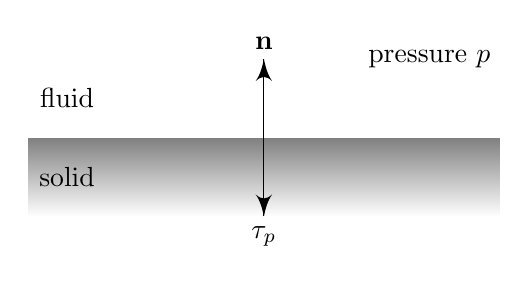
\begin{tikzpicture}
    \fill [gray, path fading=south] (0, 0) rectangle (6, -1);
    \draw [->] (3, 0) -- +(0, 1) node [above] {$\mathbf{n}$};
    \draw [->] (3, 0) -- +(0, -1) node [below] {$\tau_p$};
    \node at (0.5, -0.5) {solid};
    \node at (0.5, 0.5) {fluid};
    \node at (6, 1) [left] {pressure $p$};
  \end{tikzpicture}
\end{center}
Suppose we have a fluid with pressure $p$ acting on a surface with unit normal $\mathbf{n}$, pointing \emph{into} the fluid.

\begin{defi}[Normal stress]
  The \emph{normal stress} is
  \[
    \tau_p = -p\mathbf{n}.
  \]
\end{defi}
Gradients in pressure produce a force. For example, suppose we have a pipe, with the pump on the left:
\begin{center}
  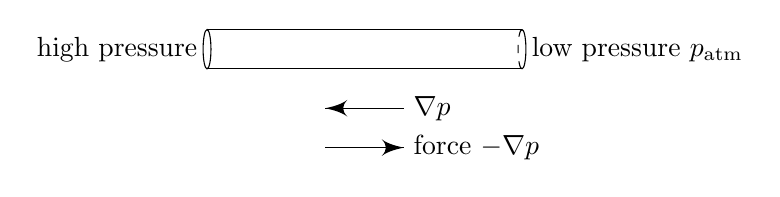
\begin{tikzpicture}
    \draw (0, 0) -- +(4, 0);
    \node at (0, 0.25) [left] {high pressure};
    \node at (4, 0.25) [right] {low pressure $p_{\mathrm{atm}}$};
    \draw (0, 0.5) -- +(4, 0);
    \draw [->] (2.5, -0.5) node [right] {$\nabla p$} -- +(-1, 0);
    \draw [->] (1.5, -1) -- +(1, 0) node [right] {force $-\nabla p$};
    \draw (0, 0.25) ellipse (0.05 and 0.25);
    \draw [dashed] (4, 0) arc (270:90:0.05 and 0.25);
    \draw (4, 0) arc (270:450:0.05 and 0.25);
  \end{tikzpicture}
\end{center}
This gives a \emph{body force} that drives the water from left to right.

\subsubsection{Tangential stress}
Consider two infinite planes with fluids in between. We keep the bottom plane at rest, and move the top plate with velocity $U$.
\begin{center}
  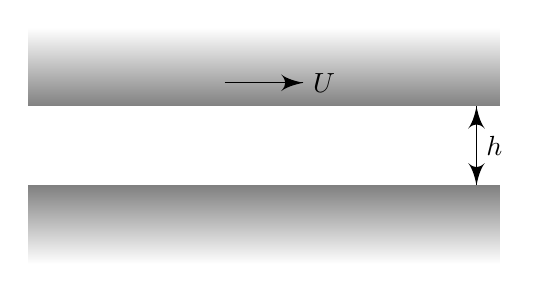
\begin{tikzpicture}
    \fill [gray, path fading=south] (0, 0) rectangle (6, -1);
    \fill [gray, path fading=north] (0, 1) rectangle (6, 2);
    \draw [->] (2.5, 1.3) -- +(1, 0) node [right] {$U$};

    \draw [<->] (5.7, 0) -- +(0, 1) node [right, pos=0.5] {$h$};
  \end{tikzpicture}
\end{center}

\begin{defi}[Tangential stress]
  The \emph{tangential stress} $\tau_s$ is the force (per unit area) required to move the top plate at speed $U$.
\end{defi}

Experimentally, we find the following.
\begin{law}
  For a Newtonian fluid, we have
  \[
    \tau_s \propto \frac{U}{h}.
  \]
\end{law}

\begin{defi}[Dynamic viscosity]
  The \emph{dynamic viscosity} $\mu$ of the fluid is the constant of proportionality in
  \[
    \tau_s = \mu \frac{U}{h}.
  \]
\end{defi}

We find the dimensions of these quantities as
\begin{align*}
  [\tau_s] &= ML^{-1} T^{-2}\\
  \left[\frac{U}{h}\right] &= T^{-1}\\
  [\mu] &= ML^{-1} T^{-1}.
\end{align*}
In SI units, $\mu$ has units $\SI{}{\kilo\gram\per\meter\per\second}$.

We have not yet said what the fluid in the middle does. It turns out this is simple: at the bottom, the fluid is constant, and at the top, the fluid moves with velocity $U$. In between, the speed varies linearly.
\begin{center}
  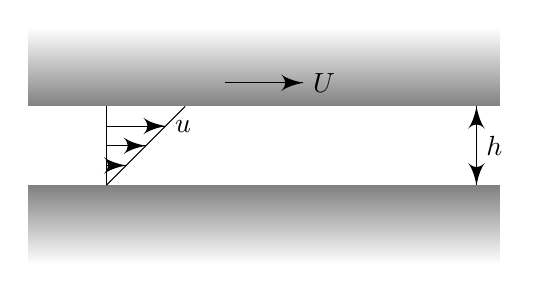
\begin{tikzpicture}
    \fill [gray, path fading=south] (0, 0) rectangle (6, -1);
    \fill [gray, path fading=north] (0, 1) rectangle (6, 2);
    \draw [->] (2.5, 1.3) -- +(1, 0) node [right] {$U$};

    \draw [<->] (5.7, 0) -- +(0, 1) node [right, pos=0.5] {$h$};

    \draw (1, 0) -- (1, 1);
    \draw (1, 0) -- (2, 1);
    \foreach \x in {0,0.25,0.5,0.75} {
      \draw [->] (1, \x) -- (1 + \x, \x);
    }
    \node at (1.75, 0.75) [right] {$u$};
  \end{tikzpicture}
\end{center}
For a general flow, let $u_T(\mathbf{x})$ be the velocity of the fluid at position $\mathbf{x}$. Then
\[
  \tau_s = \mu \frac{\partial u_T(\mathbf{x})}{\partial \mathbf{n}},
\]
and is in the direction of the tangential component of velocity.
\end{document}
